\documentclass[border=3pt]{standalone}
% Preâmbulo compartilhado pelos diagramas TikZ da aula 11 (Localização por Grade e Monte Carlo)
\usepackage[T1]{fontenc}
\usepackage[utf8]{inputenc}
\usepackage{lmodern}
\usepackage{amsmath}
\usepackage{xcolor}
\usepackage{tikz}
\usetikzlibrary{arrows.meta,angles,quotes,decorations.pathmorphing,calc,
                positioning,shapes.geometric,shapes.misc,backgrounds,fit,
                math}

% Paleta (mesma dos SVGs originais)
\definecolor{dblue}{HTML}{2A5B8C}
\definecolor{dorange}{HTML}{B3541E}
\definecolor{dgreen}{HTML}{4A7C59}
\definecolor{dred}{HTML}{9C4B4B}
\definecolor{dcream}{HTML}{F4F1EA}
\definecolor{dshade}{HTML}{DDD7C9}

% Função gaussiana (não normalizada por padrão de escala visual)
\pgfmathdeclarefunction{gauss}{3}{%
  \pgfmathparse{1/(#3*sqrt(2*pi))*exp(-((#1-#2)^2)/(2*#3^2))}%
}

% Estilos comuns (prefixo d... para não colidir com chaves internas do pgf)
\tikzset{
  >={Stealth[length=2mm]},
  dguide/.style={gray!55, dashed, line width=0.4pt},
  daxis/.style={gray!60, line width=0.7pt, ->},
  dbody/.style={fill=black!3, draw=black!80, line width=1pt},
  dacc/.style={draw=dblue, line width=1pt},
  dlbl/.style={black!55, font=\small},
  dsub/.style={black!45, font=\footnotesize},
  dstate/.style={circle, draw=black!80, fill=dcream, line width=1pt,
                 minimum size=17mm, font=\large, inner sep=1pt},
  dobs/.style={circle, draw=black!80, fill=dshade, line width=1pt,
               minimum size=14mm, font=\large, inner sep=1pt},
  dbox/.style={rounded corners=2pt, draw=black!80, fill=dcream, line width=1pt,
               align=center, inner sep=6pt},
  dop/.style={circle, draw=black!80, fill=white, line width=1pt,
              minimum size=6mm, inner sep=0pt, font=\small},
  dtrans/.style={->, dblue, line width=1pt},
  dmeas/.style={->, dorange, line width=1pt},
  dcurve/.style={line width=1pt, dblue},
  dcurveb/.style={line width=1.4pt, dorange},
}

\begin{document}
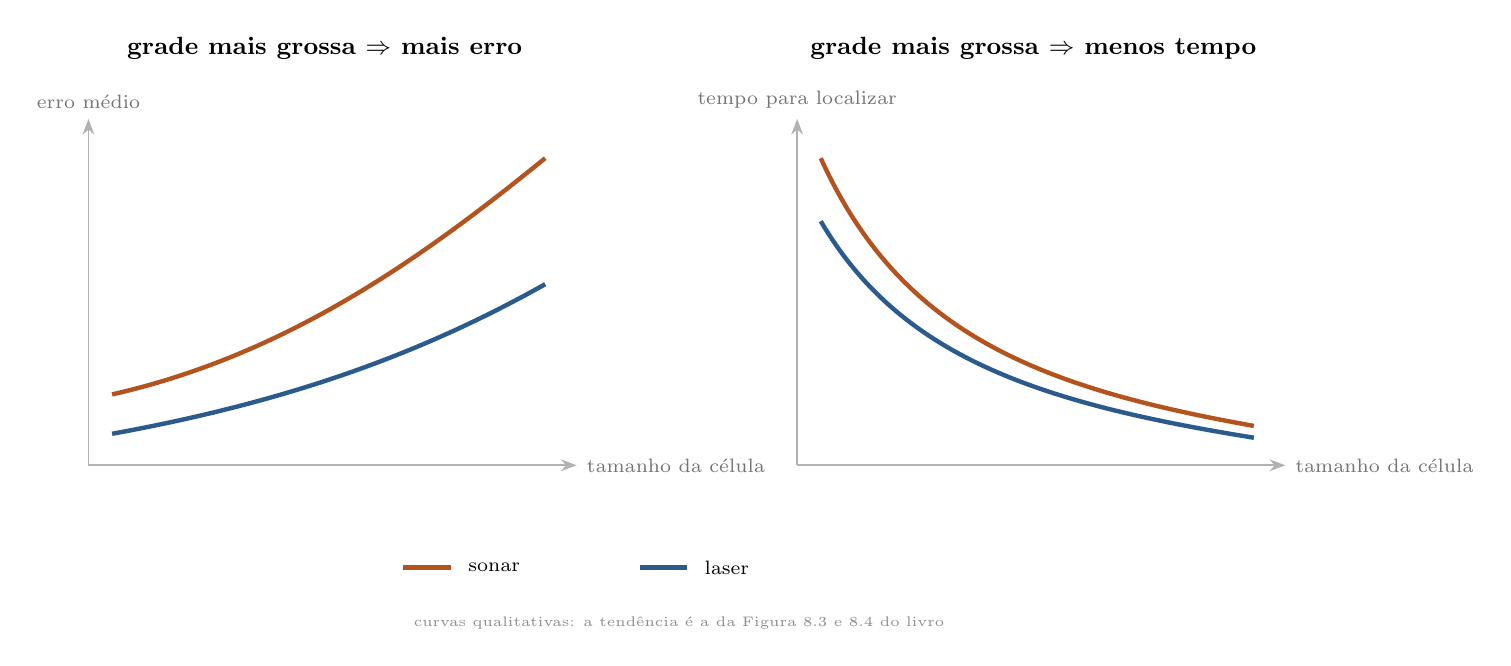
\begin{tikzpicture}[x=1cm,y=1cm]
  \newcommand{\eixos}[2]{\draw[daxis] (0,0) -- (6.2,0) node[right, dlbl, font=\scriptsize] {tamanho da célula}; \draw[daxis] (0,0) -- (0,4.4) node[above, dlbl, font=\scriptsize] {#1}; \node[font=\small\bfseries] at (3,5.3) {#2};}
  \begin{scope}
    \eixos{erro médio}{grade mais grossa $\Rightarrow$ mais erro}
    \draw[dorange, line width=1.6pt] (0.3,0.9) .. controls (2.5,1.4) and (4.2,2.6) .. (5.8,3.9);
    \draw[dblue, line width=1.6pt] (0.3,0.4) .. controls (2.5,0.8) and (4.2,1.4) .. (5.8,2.3);
  \end{scope}
  \begin{scope}[shift={(9,0)}]
    \eixos{tempo para localizar}{grade mais grossa $\Rightarrow$ menos tempo}
    \draw[dorange, line width=1.6pt] (0.3,3.9) .. controls (1.3,1.7) and (3.0,1.0) .. (5.8,0.5);
    \draw[dblue, line width=1.6pt] (0.3,3.1) .. controls (1.3,1.4) and (3.0,0.8) .. (5.8,0.35);
  \end{scope}
  \draw[dorange, line width=1.6pt] (4.0,-1.3) -- (4.6,-1.3); \node[anchor=west, font=\scriptsize] at (4.7,-1.3) {sonar};
  \draw[dblue, line width=1.6pt] (7.0,-1.3) -- (7.6,-1.3); \node[anchor=west, font=\scriptsize] at (7.7,-1.3) {laser};
  \node[dsub, font=\tiny] at (7.5,-2.0) {curvas qualitativas: a tendência é a da Figura 8.3 e 8.4 do livro};
\end{tikzpicture}
\end{document}
